\chapter{Game Theory and Cooperation: Network Imperatives and Forced Free Will} % Adjusted Title
\label{ch:GameTheory}

Having explored the emergence of structures in biological and social networks, this chapter delves into the functional necessity of cooperation within these systems, a key theme related to Principle 5 (Dual Roles of Competition and Collaboration) of the \emph{Evolution by Emergence} paradigm. We develop a formal analysis using repeated game theory, coupled with a model of agent dependency, to demonstrate how cooperation can emerge and be sustained. This analysis provides a mathematical basis for understanding Principle 6 (Constrained Agency and Network Alignment, or 'Forced Free Will'), suggesting that in interdependent networks, cooperation becomes not just a beneficial strategy but a structural imperative for long-term survival. % Revised Introduction

\section{The Repeated Game Framework}
Consider a stage game between two players, where the payoffs reflect the tension between individual gain (defection) and mutual benefit (cooperation):
\begin{itemize}
    \item \textbf{Mutual Cooperation:} Both players receive \( R \).
    \item \textbf{Unilateral Defection:} The defector receives \( T \) (the temptation payoff), while the cooperating player receives \( S \) (the sucker's payoff).
    \item \textbf{Mutual Defection:} Both players receive \( P \).
\end{itemize}
We assume \( T > R > P > S \). In a single-shot game, defection is the dominant strategy. However, in an infinitely repeated game with a discount factor \( \delta \) (where \( \delta \) is sufficiently high), cooperation can be sustained as a Nash equilibrium. This shift highlights how the network context (repeated interactions) alters optimal strategies, favoring collaboration (Principle 5). % Added link to paradigm

\subsection{The Folk Theorem}
\begin{theorem}[Folk Theorem for Repeated Games]
For an \( n \)-player repeated game with stage payoff functions \( u_i \), any feasible payoff vector \( (v_1, \dots, v_n) \) satisfying \( v_i > \bar{u}_i \) (where \(\bar{u}_i\) is the minmax payoff for player \( i \)) for all \( i \) can be sustained as a Nash equilibrium if the discount factor \( \delta \) is sufficiently high.
\end{theorem}
A strategy such as \emph{tit-for-tat with forgiveness}---where players begin by cooperating, impose brief sanctions on defectors (negative feedback, Principle 3), and then return to cooperation if the opponent reforms---illustrates how long-term cooperation becomes the rational strategy within a system valuing future interactions.

\section{The Four-Layer Dependency Model of Intelligence}
To understand \emph{why} long-term cooperation is often necessary, we introduce a four-layer dependency model. This model articulates how an agent's survival depends on multiple interdependent levels (Principle 4: Interdependence), providing context for the constraints agents face (Principle 6):
\begin{enumerate}
    \item \textbf{Layer 1: Intelligence.}   
    The cognitive core, such as human reasoning or an AI's decision-making process.
    \item \textbf{Layer 2: Substrate.}   
    The physical embodiment (e.g., human body or AI hardware) that enables intelligence.
    \item \textbf{Layer 3: Resources.}   
    Consumable inputs (e.g., food, energy, water) required to maintain the substrate.
    \item \textbf{Layer 4: Fundamental Sources.}   
    The ultimate origins of these resources (e.g., sunlight, soil, planetary processes).
\end{enumerate}
\begin{center}
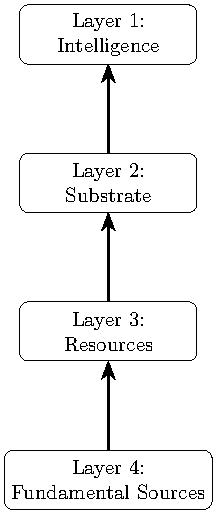
\includegraphics{docs/figures/layers} 
\end{center}
Because agents often share resources (Layer 3) that are derived from common fundamental sources (Layer 4), their fates are linked through interdependence (Principle 4). Actions that overexploit these shared layers jeopardize not only the physical substrate but ultimately the capacity for intelligence itself, imposing network constraints (Principle 6). % Added links to paradigm

\section{Integrating Resource Dynamics with the Four-Layer Model}
We model the instantaneous payoff of an agent \( i \) as:
\[
u_i(t) = f(c_i(t)) \cdot g(q(t)),
\]
where:
\begin{itemize}
    \item \( c_i(t) \) is the consumption of resources by agent \( i \) at time \( t \).
    \item \( f(c) \) is an increasing function representing the benefits from consumption.
    \item \( g(q) \) is a function of the resource state \( q(t) \), reflecting the health of the shared resource base (Layer 3/4). \( g(q) \) is near unity when resources are abundant and declining as resources degrade.
\end{itemize}
The resource dynamics are given by:
\[
q(t+1) = q(t) + R_{\text{regen}} - \sum_{i=1}^{N} c_i(t),
\]
where \( R_{\text{regen}} \) denotes the natural regeneration rate. Overconsumption by any agent depletes \( q(t) \), thus lowering the benefits \( g(q) \) for all agents connected through this shared resource. This feedback loop (Principle 3) illustrates the interdependence (Principle 4) and highlights why agents, to maximize long-term payoffs, must cooperate to restrain consumption and sustain the substrate essential for intelligence. This constraint forces alignment with sustainable behavior (Principle 6). % Added links to paradigm

\section{Network Perspective and Edge Restoration}
We can represent the system as a graph \( G = (V,E) \), where nodes are agents and edges represent cooperative relationships (Principle 2: Dynamic Networks). In this framework:
\begin{itemize}
    \item When an agent defects (violating Principle 5's collaborative aspect), its corresponding cooperative link may break with probability \( p \).
    \item A forgiveness mechanism (a form of adaptive feedback, Principle 3) can restore these links with probability \( r \).
\end{itemize}
The steady-state fraction of active cooperative links, \( \pi \), is approximated by:
\[
\pi = \frac{r}{p + r}.
\]
A robust cooperative network (high \( \pi \)) is crucial for maintaining the shared resource base and, by extension, the integrity of the four-layer structure, demonstrating the importance of network topology for system function (Principle 9). % Added link to paradigm

\section{Decentralized Rules for Sustaining Cooperation}
Based on our analysis, the following decentralized guidelines, reflecting local interactions driving global order (Principle 1), are proposed to sustain cooperation within the network:
\begin{enumerate}
    \item \textbf{Default Cooperation:} Begin interactions by cooperating unless defection is evident (aligning with Principle 5).
    \item \textbf{Observation and Memory:} Monitor local behavior and maintain a short-term record of interactions (information processing).
    \item \textbf{Conditional Punishment:} Impose temporary sanctions on defectors to signal that defection carries a cost (negative feedback, Principle 3).
    \item \textbf{Forgiveness:} Restore cooperative ties once the defector resumes cooperative behavior (adaptive feedback, Principle 3).
    \item \textbf{Resource Awareness:} Recognize that long-term benefits depend on preserving shared resources (acknowledging interdependence, Principle 4), thereby motivating restraint (aligning with network constraints, Principle 6).
\end{enumerate}
These local rules help create a globally robust network in which cooperation emerges as the rational long-term strategy, illustrating the core ideas of the Evolution by Emergence paradigm. % Adjusted paragraph

\section{Discussion and Implications}
Our integrated framework demonstrates that cooperation can emerge as a stable outcome under repeated interactions, provided agents account for both immediate payoffs and the long-term integrity of the shared resource base (Principle 4: Interdependence). This formalizes the collaborative aspect of Principle 5 and provides a mechanism for Principle 6 (Forced Free Will/Network Alignment). However, several caveats merit discussion:
\begin{itemize}
    \item \textbf{Model Limitations:} The theoretical models assume rationality and simplified dynamics that may not capture all real-world complexities (acknowledging limits, relevant to Principle 8 and 9).
    \item \textbf{Is-Ought Gap:} While the analysis shows that cooperation is a sustainable strategy, additional ethical reasoning is required to justify its normative superiority (relevant to Principle 10).
    \item \textbf{Empirical Validation:} The predictions must be tested against observations from ecological, social, and technological systems.
\end{itemize} % Added links to paradigm

\section{Conclusion}
By integrating repeated game theory with the four-layer dependency model and network analysis, this chapter has formally illustrated key principles of the Evolution by Emergence paradigm. We have shown that cooperation (Principle 5) is not only strategically optimal in repeated interactions but often structurally necessary due to interdependence (Principle 4). When agents recognize their reliance on shared resources and substrates, the network dynamics constrain their choices, forcing alignment towards sustainable, cooperative behavior (Principle 6). This formal analysis, while subject to model limitations and normative debates, provides a robust framework for understanding the emergence of cooperation as a fundamental aspect of evolving networks in both biological and artificial systems. % Revised Conclusion
\cleardoublepage
